\begin{mainquestion}{dependentsource01}{Working with Dependent Sources}
Consider the circuit below, which contains a dependent source.
\begin{center}
    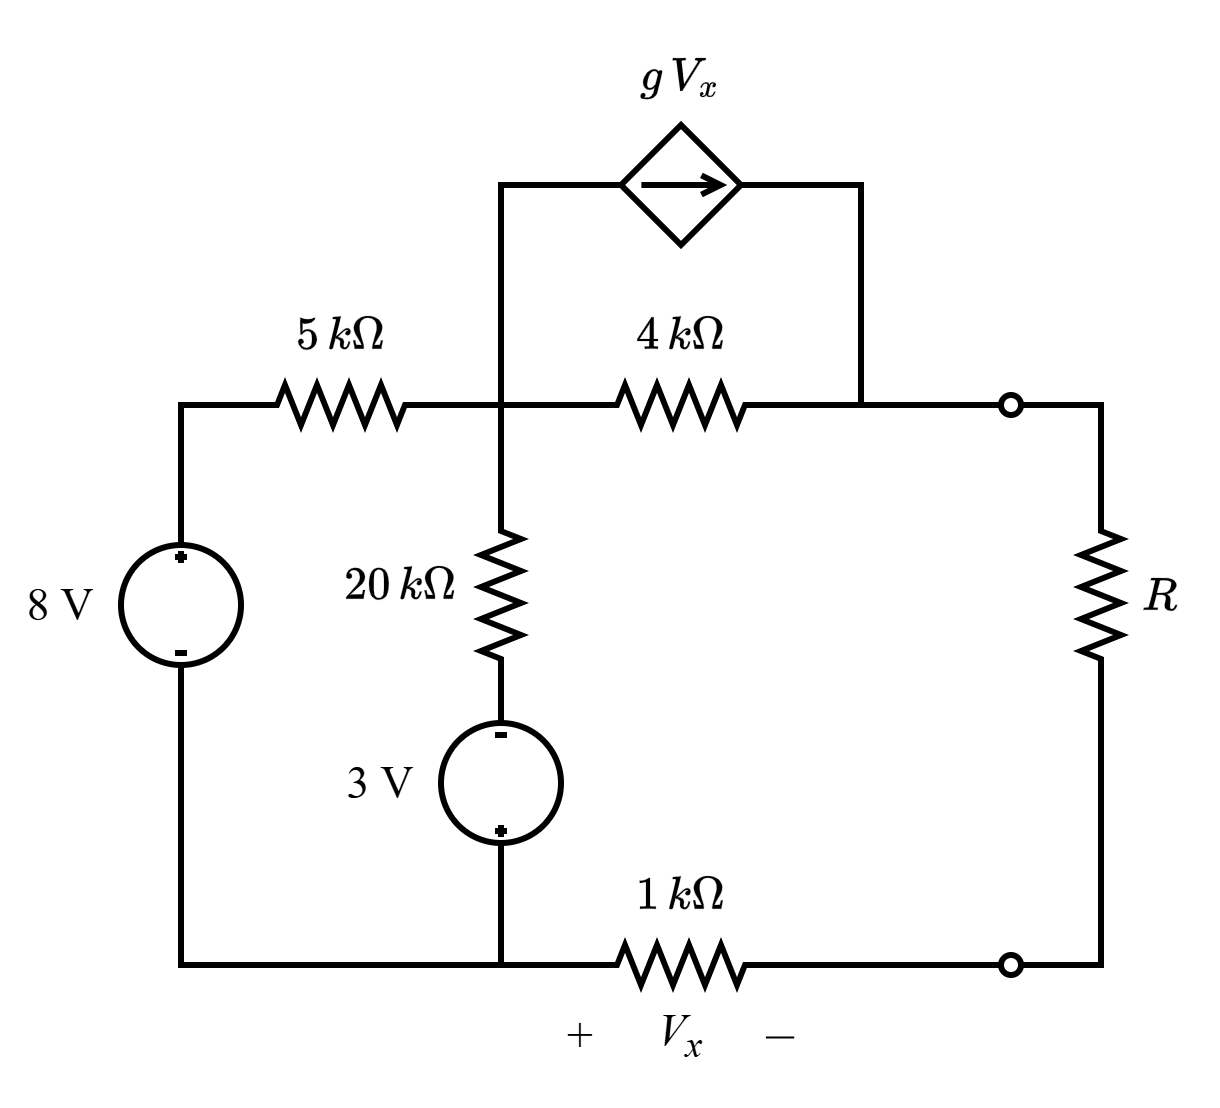
\includegraphics[width=4in]{figure.png}
\end{center}

\begin{partquestion}{units}{What type of dependent source is shown here?  What are the units of $g$?}
\begin{answer}
This is a voltage controlled current source (VCCS).  The variable $g$ is one of transconductance, and is measured in siemens (S). 
\end{answer}
\end{partquestion}

\begin{partquestion}{xform}{Perform a single source transformation with the dependent source, and redraw the circuit.}
\begin{answer}
Because we are not destroying our definition of $V_x$, we can source transform the parallel combination of the current source and the $4\,k\Omega$ resistor into a Th\'evenin equivalent, with a voltage value of $(gV_x)(4000)$ in series with a resistor of value $4\,k\Omega$, as shown below.
\begin{center}
    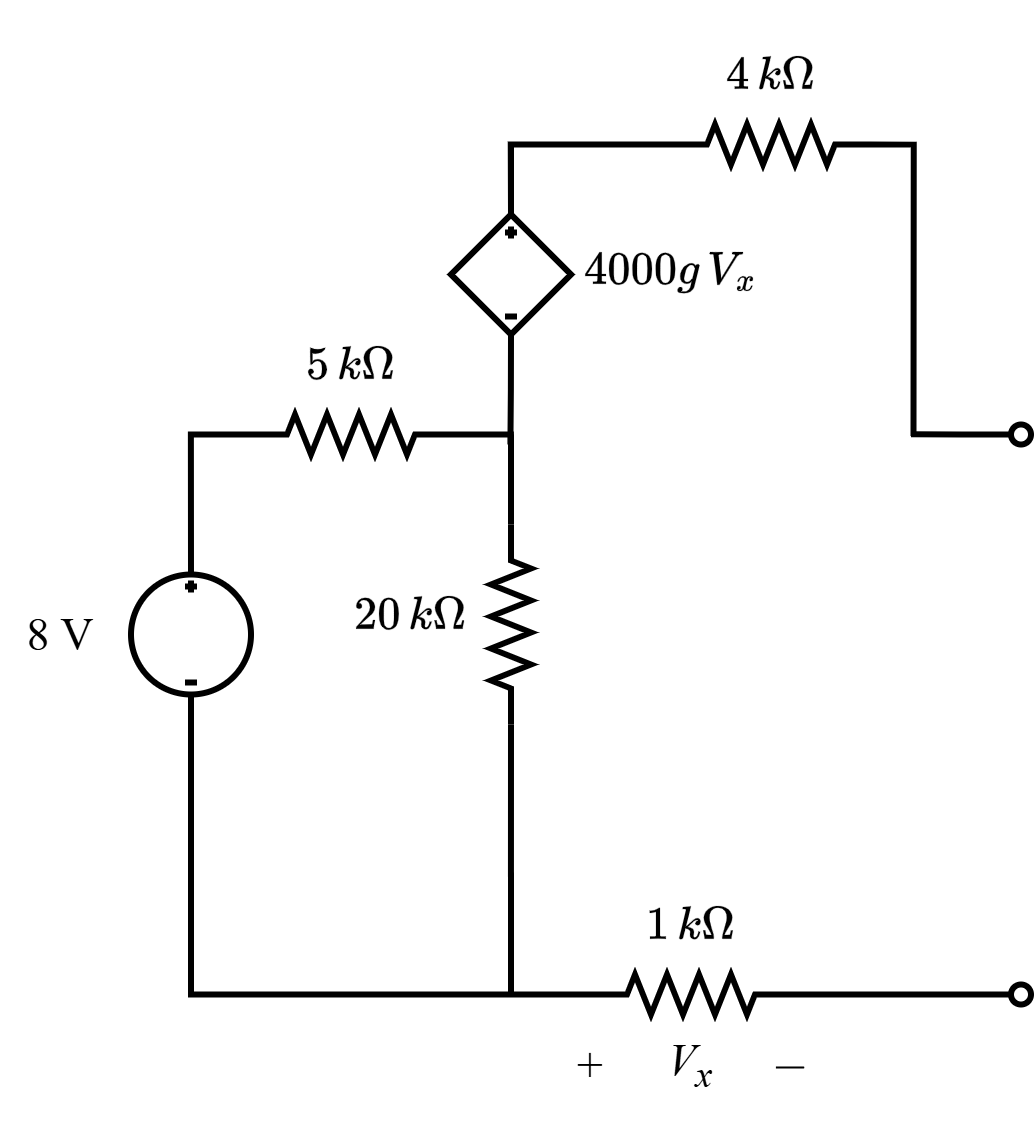
\includegraphics[width=2in]{figure2.png}
\end{center}
\end{answer}
\end{partquestion}

\begin{partquestion}{vth}{Use superposition to find $V_\mathrm{th}$ in terms of $g$.  How does $V_\mathrm{th}$ vary with $g$?}
\begin{answer}
We need to determine the effects of each independent source on the open-circuit voltage at the load terminals by zeroing out the remaining independent sources.  The dependent source must NOT be zeroed out, and remains present during each (of two) analyses. We start with the 8 V supply present and the 3 V supply zeroed out, leading to the following circuit:
\begin{center}
    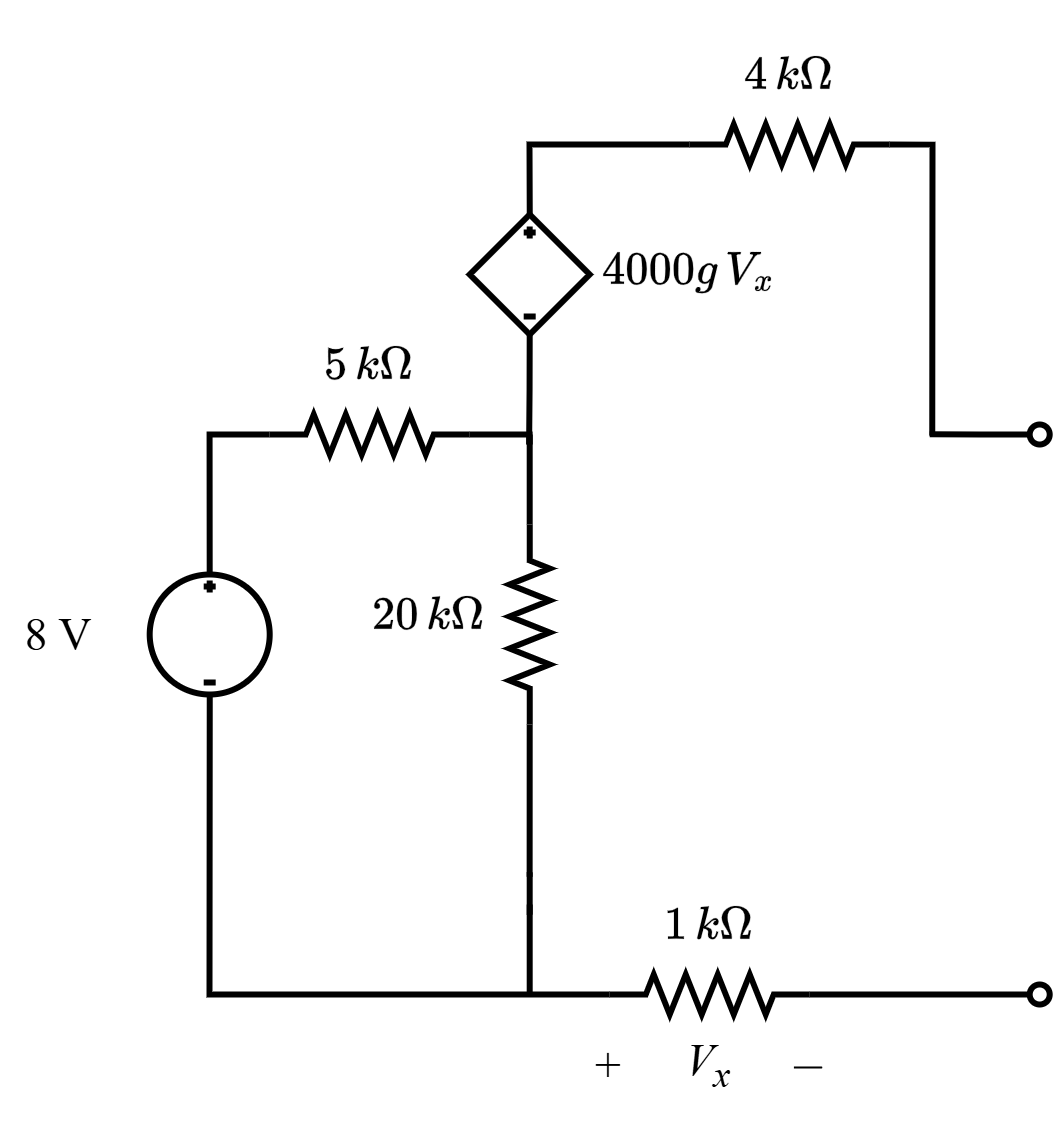
\includegraphics[width=2in]{figure3.png}
\end{center}
Note that in this transformed circuit, with the load open circuited, there is no current flow through either the \qty{1}{\kilo\ohm} or the \qty{4}{\kilo\ohm} resistor.  By Ohm's Law, there must therefore be no voltage drop across these resistors, which forces $V_x=0$, and consequently the dependent source has a value of \qty{0}{\volt}.  The only contribution is from the voltage across the \qty{20}{\kilo\ohm} due to the 8 V source.  This implies
\begin{align*}
V_{oc1}=(\qty{8}{\volt})\frac{\qty{20}{\kilo\ohm}}{\qty{5}{\kilo\ohm}+\qty{20}{\kilo\ohm}}=\qty{6.4}{\volt}
\end{align*}

Next we use the 3 V supply with the 8 V supply zeroed out, leading to the following circuit:
\begin{center}
    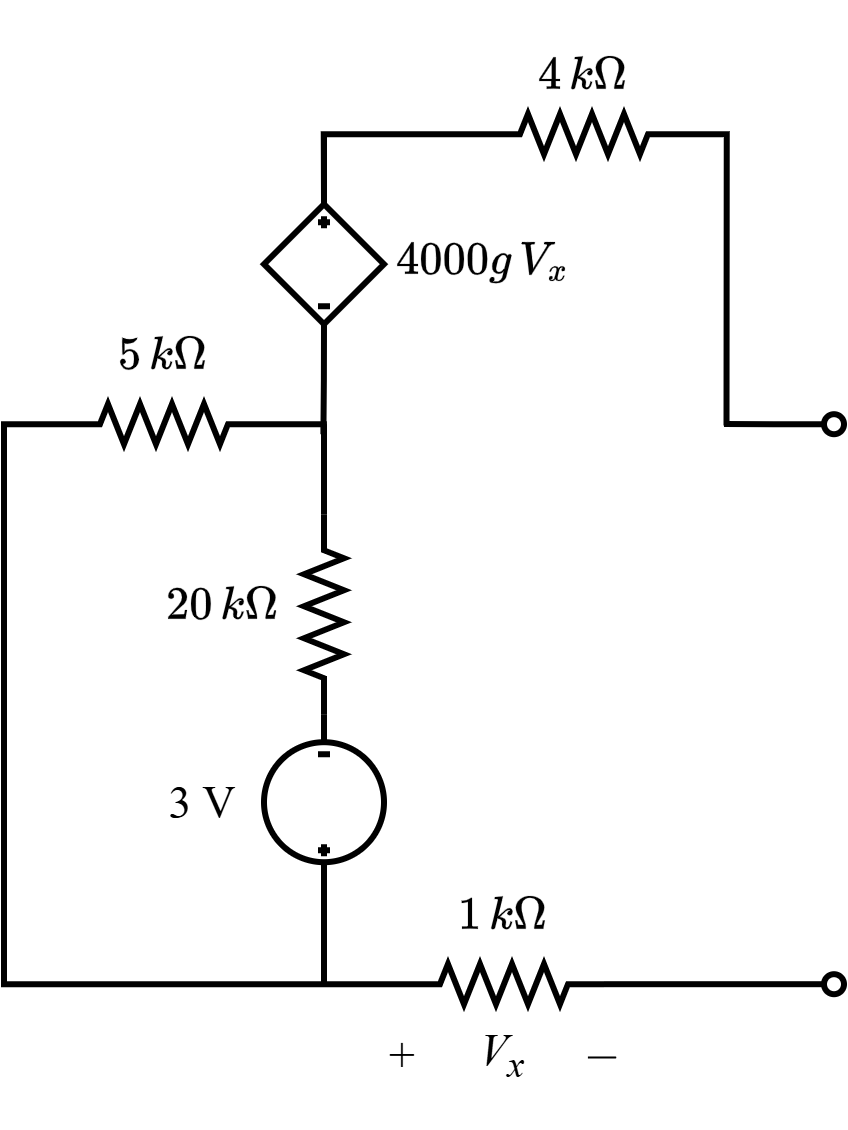
\includegraphics[width=2in]{figure4.png}
\end{center}
Again in this transformed circuit, there is no current flow through either the \qty{4}{\kilo\ohm} or the \qty{1}{\kilo\ohm} resistor, nor the dependent source in this open-circuit configuration.  The only contribution is from the voltage across the \qty{20}{\kilo\ohm} due to the 3 V source and $\qty{-3}{volt}$ in series. This implies
\begin{align*}
V_{oc2}=(\qty{3}{\volt})\frac{\qty{20}{\kilo\ohm}}{\qty{5}{\kilo\ohm}+\qty{20}{\kilo\ohm}}-\qty{3}{\volt}=\qty{-0.6}{\volt}
\end{align*}
By superposition, we have
\[
V_{\mathrm{th}}=V_{oc}=V_{oc1}+V_{oc2}=\qty{6.4}{\volt}-\qty{0.6}{\volt}=\qty{5.8}{\volt}
\]
\end{answer}
\end{partquestion}

\begin{partquestion}{rth}{Find $R_\mathrm{th}$ in terms of $g$.  How does $R_\mathrm{th}$ vary with $g$?}
\begin{answer}
To find $R_\mathrm{th}$, we zero out all independent sources, and are left with the following circuit.
\begin{center}
    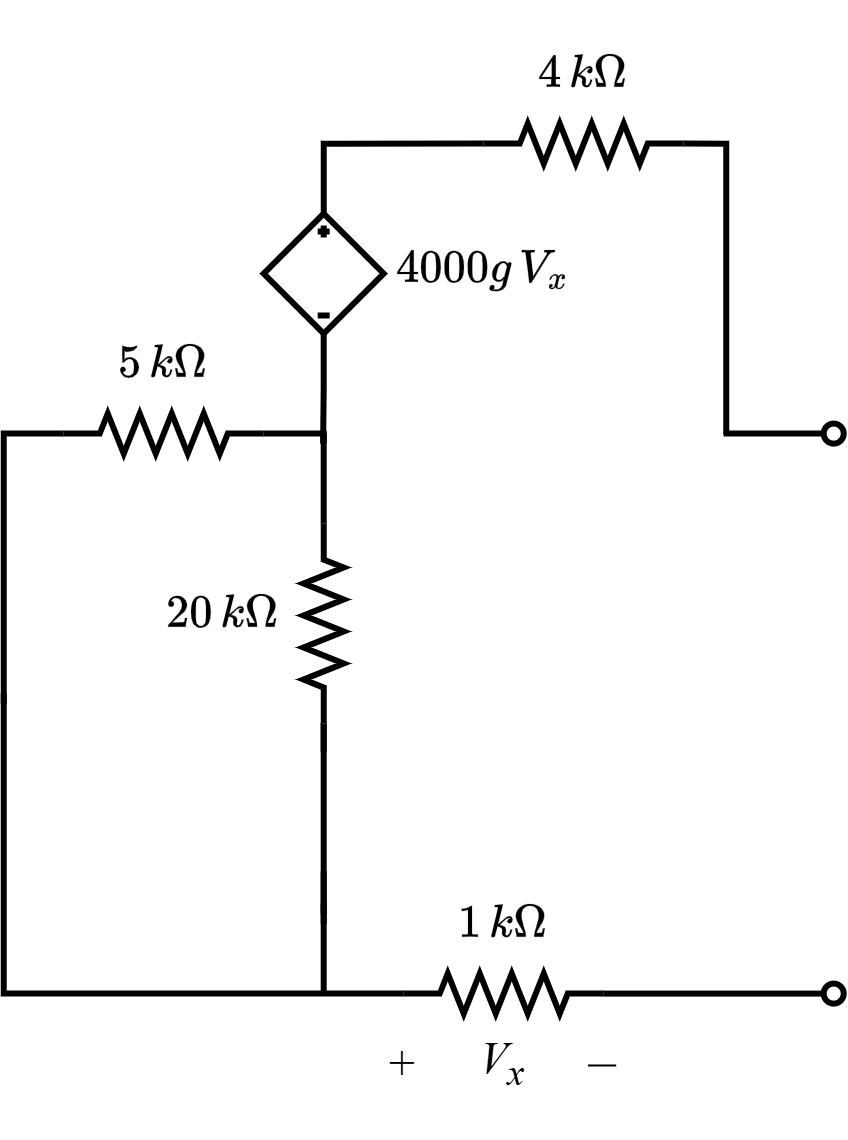
\includegraphics[width=2in]{figure5.png}
\end{center}
The presence of the dependent source prevents us from simply being able to read the resistance seen at the load terminals by inspection, and we must use the test source method with $v_x$ and $i_x$.  The parallel \qty{5}{\kilo\ohm} and \qty{20}{\kilo\ohm} can be added to the $4\,k\Omega$ resistor to find an equivalent resistance of:
\[
\qty{5}{\kilo\ohm}||\qty{20}{\kilo\ohm}+\qty{4}{\kilo\ohm}=\frac{\qty{250}{\kilo\ohm}\cdot\qty{20}{\kilo\ohm}}{\qty{5}{\kilo\ohm}+\qty{20}{\kilo\ohm}}+\qty{4}{\kilo\ohm}=\qty{4}{\kilo\ohm}+\qty{4}{\kilo\ohm}=\qty{8}{\kilo\ohm}
\]
Now we can input a test source to create the following circuit:
\begin{center}
    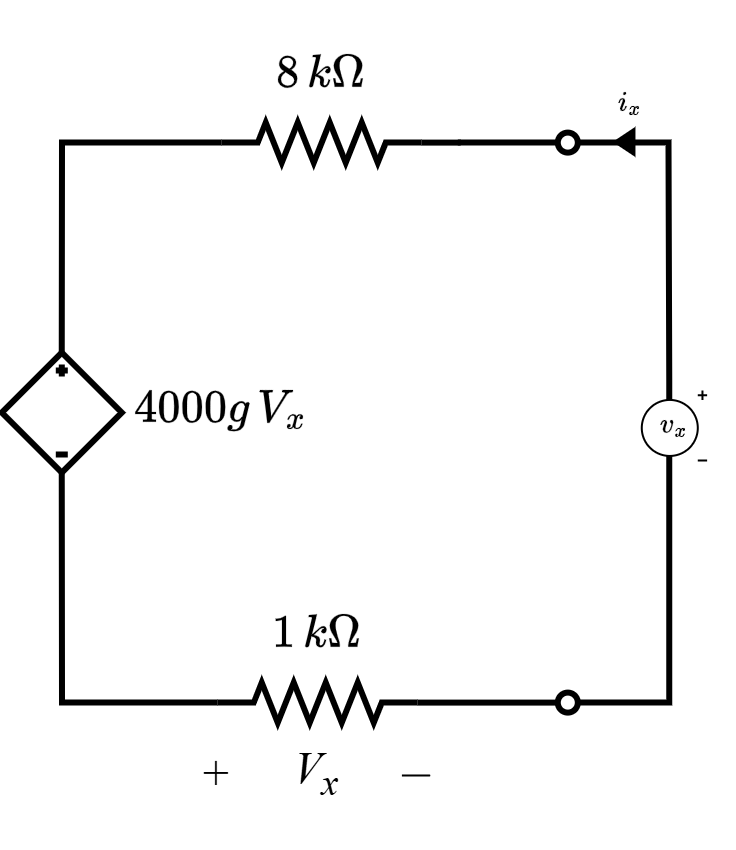
\includegraphics[width=2in]{figure6.png}
\end{center}KVL around the loop gives:
\[
(\qty{8}{\kilo\ohm})i_x + 4000gV_x+V_x-v_x=0
\]
Since $V_x = (\qty{1}{\kilo\ohm})i_x$, we can write this as:
\[
(\qty{8}{\kilo\ohm})i_x + (4000g+1)(\qty{1}{\kilo\ohm})i_x-v_x=0
\]
and
\[
\frac{v_x}{i_x}\triangleq R_{\mathrm{th}}=\qty{8}{\kilo\ohm}+(4000g+1)(\qty{1}{\kilo\ohm})=(9+4000g)\,\qty{}{\kilo\ohm}
\]
\end{answer}
\end{partquestion}

\begin{partquestion}{rl}{What is the value of $R$ that results in the maximum power being transferred to this load?}
\begin{answer}
For maximum power transfer, $R=R_{\mathrm{th}}$ so
\[
R=(9+4000g)\,\qty{}{\kilo\ohm}
\]
\end{answer}
\end{partquestion}

\begin{partquestion}{pl}{Describe how increasing $g$ affects $P_{L,\max}$, the maximum power dissipated in the load.  Briefly justify your answer.}
\begin{answer}
The maximum power delivered is
\[
P_{L,\max}= \frac{V_{\mathrm{th}}^2}{4R_{\mathrm{th}}}
\]
From part (\cref{prob:dependentsource01:vth}) we found the voltage $V_{\mathrm{th}}$ did not depend on $g$. In part (\cref{prob:dependentsource01:rth}) we found $R=R_{\mathrm{th}}$ increased as $g$ increased.  It follows that $P_{L,\max}$, given $R_{\mathrm{th}}$ in its denominator, must decrease as $g$ increases.
\end{answer}
\end{partquestion}

\begin{partquestion}{numbers}{Evaluate numerical values for $V_\mathrm{th}$, $R_\mathrm{th}$, $R$, $P_{L,\max}$ and load current $I_L$ when $g=0.002$.}
\begin{answer}
\begin{align*}
&V_{\mathrm{th}}=\qty{5.8}{\volt}\\
&R_{\mathrm{th}}=9+4000\cdot0.002=\qty{17}{\kilo\ohm}\\
&R=R_{\mathrm{th}}=\qty{17}{\kilo\ohm}\\
&P_{L,\max}= \frac{(\qty{5.8}{\volt})^2}{4\cdot\qty{17}{\kilo\ohm}}=\qty{0.495}{\milli\watt}\\
&I_L=\frac{V_{\mathrm{th}}}{2R_{\mathrm{th}}}=\frac{\qty{5.8}{\volt}}{2\cdot\qty{17}{\kilo\ohm}}=\qty{0.17}{\milli\ampere}
\end{align*}
\end{answer}
\end{partquestion}

\begin{partquestion}{negative}{Suppose the polarity of the controlling voltage $V_x$ is reversed while everything else in the circuit remains unchanged. Explore how this change affects the Th\'evenin equivalent seen by the load as $g$ varies. Discuss any interesting or unexpected observations.}
\begin{answer}
The problem is the same, but $V_x$ is now replaced by $-V_x$, which is equivalent to $g$ being replaced by $-g$.  This will of course still have no impact on $V_{\mathrm{th}}$, but now 
\[
R_{\mathrm{th}}=(9-4000g)\,\qty{}{\kilo\ohm}
\]
Note that now, when $g>\frac{9}{4000}=0.00225$, $R_{\mathrm{th}} < 0$! This is a direct result of an active circuit feeding energy back into the load terminals.  It may be interesting to know that when $R_{\mathrm{th}} < 0$, the standard passive maximum-power-transfer result $R=R_{\mathrm{th}} < 0$ is no longer applicable to a positive physical load! You may get a chance to explore these situations with "negative resistance" a bit further in EE101B.
\end{answer}
\end{partquestion}
\end{mainquestion}